\documentclass[xcolor=dvipsnames]{beamer}
%%%%%%%%%%%%%%%%%%%%%%%%%%%%%%%%%%%%
%
% Packages
%
%%%%%%%%%%%%%%%%%%%%%%%%%%%%%%%%%%%%
\usepackage{hyperref}
\usepackage{caption}
\usepackage{subcaption}
\usepackage{amsmath,amsfonts,amssymb}
\usepackage{lmodern}
\usepackage{graphicx}
\usepackage{caption}
\setcounter{MaxMatrixCols}{14}
\usepackage{multicol}
\usepackage{etoolbox}
\usepackage{bibentry}
\usepackage{dsfont}

\usepackage[utf8]{inputenc}
\usepackage[T1]{fontenc}
\usepackage[french]{babel}

\usepackage{babel,blindtext}
\usepackage{color}
\DeclareMathOperator*{\argmin}{arg\,min}
\usepackage{tikz}
\usetikzlibrary{shapes,shadows,arrows}

\setbeamercovered{dynamic}
\useinnertheme{rectangles}

\usepackage{media9}

\usepackage[style=authortitle]{biblatex}
%%%%%%%%%%%%%%%%%%%%%%%%%%%%%%%%%%%%
%
% Theme
%
%%%%%%%%%%%%%%%%%%%%%%%%%%%%%%%%%%%%
\usetheme{Boadilla}
\usecolortheme[named=Brown]{structure}
\usetheme[height=7mm]{Rochester}

\title{Control of prosumer Networks}
\author[N. Gensollen]{\textbf{Nicolas Gensollen}, Vincent Gauthier, Monique Becker, Michel Marot}
\institute[TSP]{
  CNRS SAMOVAR, Telecom SudParis\\
  Institut Mines\-Telecom\\[1ex]
  \texttt{nicolas.gensollen@telecom-sudparis.eu}
}
\date{11 March 2016}

%%%%%%%%%%%%%%%%%%%%%%%%%%%%%%%%%%%%
%
% Main Document
%
%%%%%%%%%%%%%%%%%%%%%%%%%%%%%%%%%%%%
\addbibresource{beamer.bib}
\begin{document}

\begin{frame}
	%\bibliographystyle{plain}
	%\nobibliography{beamer}
		\titlepage
\end{frame}
%%%%%%%%%%%%%%%%%%%%%%%%%%%%%%%%%%%%
%
% Slides Title
%
%%%%%%%%%%%%%%%%%%%%%%%%%%%%%%%%%%%%
\begin{frame}
	\frametitle{Global introduction}
	
	\begin{columns}
		\begin{column}{.6\textwidth}
			\begin{itemize}
				\item PhD in SAMOVAR
				\item Background : Telecom, computer science, complex systems
				\item Smart grid : new and cross disciplines 
				\item Complex system approach of prosumer managment in the smart grid
				\item Prosumer = PROducer + conSUMER
				%\item Chapter 1 : Forming stable aggregations of prosumers for energy markets
				%\item Chapter 2 : Control of prosumer networks
			\end{itemize}
		\end{column}
		\begin{column}{.4\textwidth}
			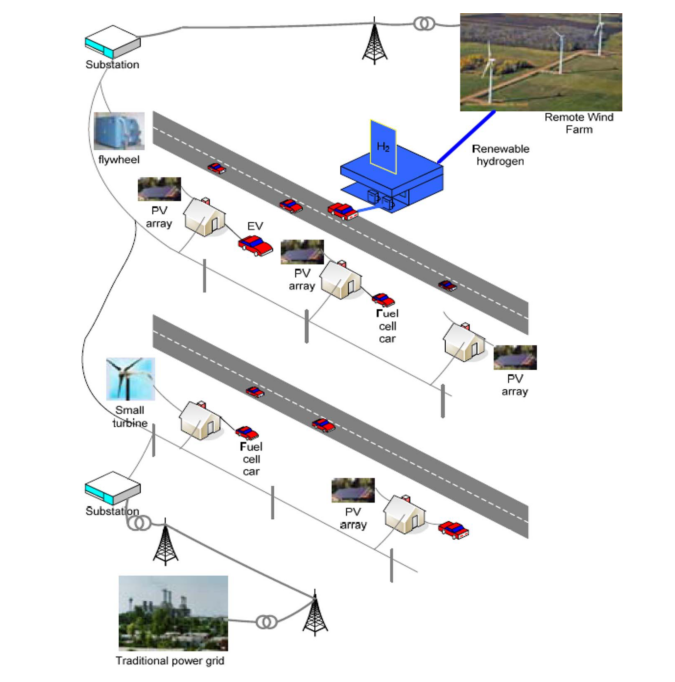
\includegraphics[scale=.3]{smart_grid}
		\end{column}
	\end{columns}
\end{frame}

\begin{frame}
	\frametitle{Smart Grid as a complex system}
	
	\begin{columns}
		\begin{column}{.5\linewidth}
			\begin{itemize}
				\item Multiple layers
				\item Decentralized production
				\item Extensive use of renewables
				\item Stochasticity
				\item Use of different storage technologies
				\item Electric vehicles
				\item Complex applications :
				\begin{itemize}
					\item Dynamic pricing
					\item Demand Side Managment
					\item V2G...
				\end{itemize}
			\end{itemize}		
		\end{column}
		\begin{column}{.5\linewidth}		
			\begin{figure}
				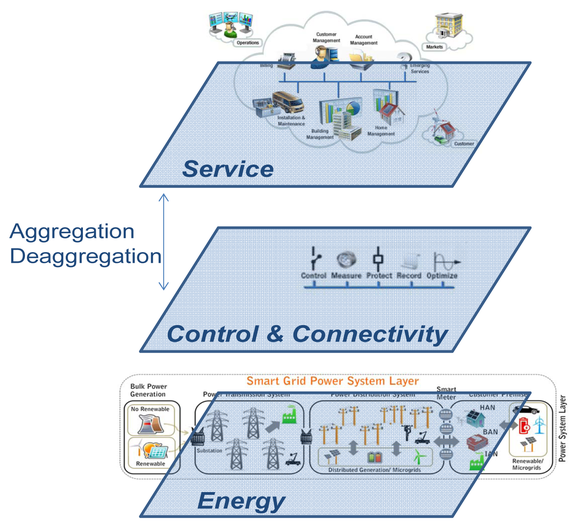
\includegraphics[scale=2]{smart_grid_3}
			\end{figure}
		\end{column}
	\end{columns}
\end{frame}

\begin{frame}
	\frametitle{Scenario}
	
	\begin{columns}
		\begin{column}{.4\linewidth}
			\begin{scriptsize}
			\begin{itemize}
				\item Smart grid with decentralized production
				\item Production and Consumption are stochastic
				\item Generators and loads are not fixed
				\item Synchronization at $ \Omega=50Hz $
				\item Production / Consumption imbalance ==> desynchronization
				\item Restaure synchrony by injecting or withdrawing power from the grid
				\item Use of storage (fixed, V2G)
				\item How to place these elements ?
			\end{itemize}
			\end{scriptsize}
		\end{column}
		\begin{column}{.6\linewidth}
			\begin{figure}
				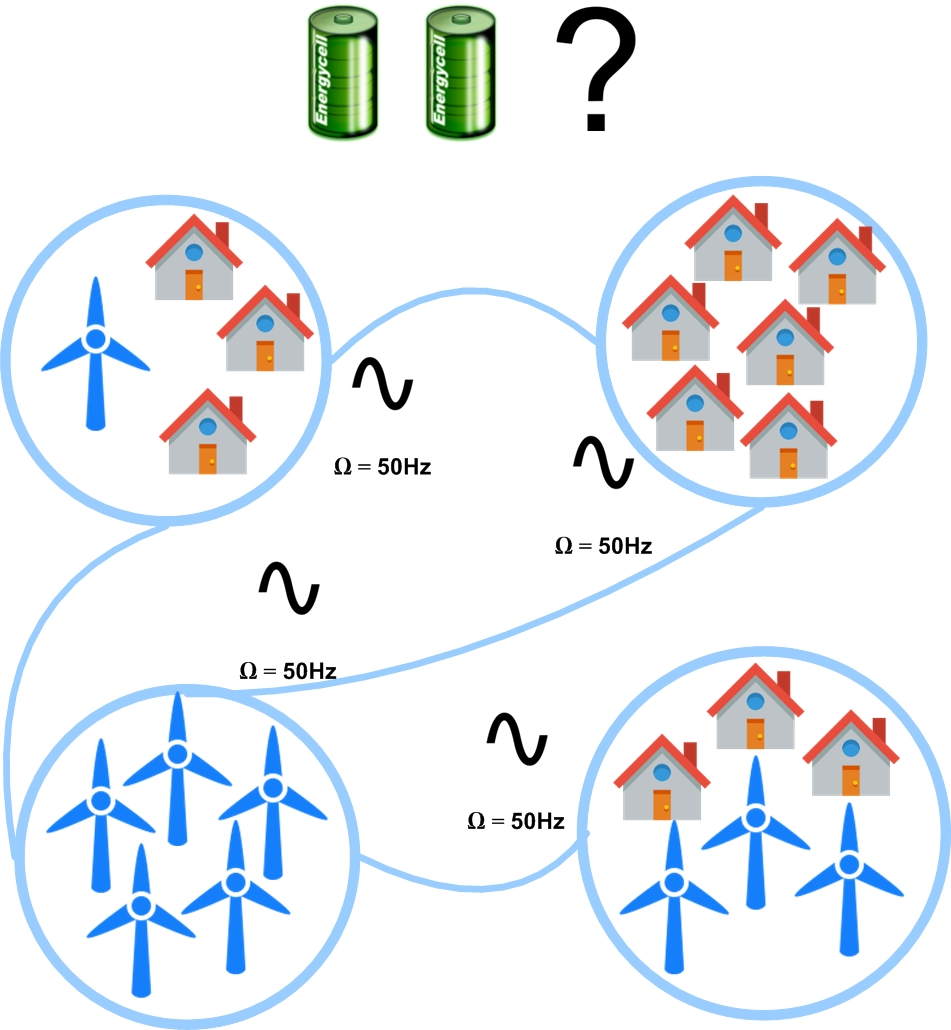
\includegraphics[scale=.3]{prosumer.jpg}
			\end{figure}
		\end{column}
	\end{columns}
\end{frame}

\begin{frame}
	\frametitle{Outline}
	\tableofcontents
\end{frame}


\section{Kuramoto Model}

\begin{frame}
	\frametitle{Simple Kuramoto Model}
	
	\begin{itemize}
		\item Widely used model to study synchronization in complex networks
		\item Nodes = oscillators with phase angles $ \theta_i $ and frequencies $ \dot{\theta}_i $
		\item Nodes have a natural frequency $\omega_i $
		\item Interconnected through a network $G=(V,E)$ of N nodes
		\item Each node's frequency is affected by its neighbors (K is the coupling strength) :
	\end{itemize}
	\begin{center}
		\[ \dot{\theta}_i = \omega_i + \frac{K}{N} \sum_{i=1}^{N} sin(\theta_j - \theta_i) \]
	\end{center}
	What is synchronization ?
	\begin{itemize}
		\item Synchronization : $ \forall i,\ \dot{\theta}_i = \omega_{SYNC} $
		\item Phase cohesiveness : $ \forall (i,j),\ \exists \gamma \in [0,\frac{\pi}{2}[,\ \vert \theta_i - \theta_j \vert \leq \gamma $
	\end{itemize}	
\end{frame}



\begin{frame}
	\frametitle{Synchronization in Kuramoto Model}
	
	\begin{itemize}
		\item Can we predict wether a given system will synchronize or not ?
		\item The network synchronizes if $ \Vert L^{\dagger} \omega \Vert_{\infty,E} \leq sin(\gamma) $ \footfullcite{Dorfler2013}
		\item Where $L^{\dagger}$ is the pseudo-inverse of the network Laplacian L
		\item $ \omega = \{ \omega_1, \omega_2,..., \omega_N \}$
		\item $ \Vert x \Vert_{\infty,E} = max_{i,j} \Vert x_i - x_j \Vert $ such that edge $(i,j)$ in E
		\item In our case : $ K \geq \frac{N \Vert L^{\dagger} \omega \Vert_{\infty,E}}{sin \gamma} $
	\end{itemize}
\end{frame}

%\begin{frame}
%	\frametitle{Synchronization in Kuramoto Model}
%	
%\begin{center}
%\includemedia[
%  width=\textwidth,height=.7\textwidth,
%  activate=pageopen,
%  flashvars={
%    modestbranding=1 % no YT logo in control bar
%   &autohide=1       % controlbar autohide
%   &showinfo=0       % no title and other info before start
%  }
%]{}{http://www.youtube.com/v/WO793FIkOPM?rel=0}   % Flash file
%\end{center}
%
%\end{frame}

\begin{frame}
	\frametitle{Synchronization in Kuramoto Model}

	\begin{center}
		\includemedia[
  			width=\linewidth,
  			height=0.8\linewidth,
  			activate=pageopen,
 			addresource=no_sync_2.MP4,
  			flashvars={source=no_sync_2.MP4}
		]{}{VPlayer.swf}
	\end{center}

\end{frame}

\begin{frame}
	\frametitle{Model power grid with Kuramoto}
	
	\begin{scriptsize}
	\begin{columns}
		\begin{column}{.45\textwidth}
			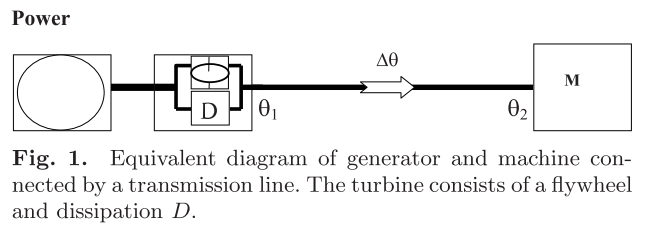
\includegraphics[scale=.45]{line}
		\end{column}
		\begin{column}{.55\textwidth}
			\begin{itemize}
				\item OBJ : Achieve synchronization at $ \Omega = 50Hz $
				\item Rewrite $ P_{source} = P_{diss} + P_{acc} + P_{trans} $ in terms of frequencies and phase angles :
				\begin{itemize}
					\item $ P_{diss} = K_D \dot{\theta}_i^2	$
					\item $ P_{acc} = \frac{1}{2}I\frac{d}{dt}\dot{\theta}_i^2 $	
					\item $P_{trans}(i \rightarrow j) = -P_{ij}^{MAX} sin(\theta_j-\theta_i) $ 
				\end{itemize}
			\end{itemize}
		\end{column}
	\end{columns}
	\begin{itemize}
		\item Dynamics is expressed in terms of the deviations from $ \Omega $ (see \footfullcite{Filatrella2008})
		\item $ \ddot{\theta}_i \sim \psi_i - \alpha_i \dot{\theta}_i + \sum_{j}K_{ij} sin(\theta_j-\theta_i) $
		\item Where :
			\begin{itemize}
				\item $ \alpha = \frac{2K_D}{I} $ : dissipation
				\item $ K_{ij} = \frac{P_{ij}^{MAX}}{I\Omega} $ : coupling
				\item $ \psi_i = \left[ \frac{P_{S,i}}{I\Omega} - \frac{K_D\Omega}{I} \right] $ : power distribution
			\end{itemize} 
		\item Small angle differences : $sin(\theta_j - \theta_i) \sim \theta_j - \theta_i $
		\item Dynamics can be written in matrix form : $Y(t+\Delta t) = A Y(t)$
	\end{itemize}
	
	\end{scriptsize}
\end{frame}

%\begin{frame}
%	\frametitle{In matrix form}
%	\begin{small}
%	\begin{itemize}
%		\item Small angle differences : $sin(\theta_j - \theta_i) \sim \theta_j - \theta_i $
%		\item Dynamics can be written in matrix form :
%	\end{itemize}
%	\end{small}
%	\[ \left( \begin{array}{ccc}
%\theta_1(t+\Delta t) \\
%\theta_2(t+\Delta t) \\
%\vdots \\
%\theta_N(t+\Delta t) \\
%\dot{\theta}_1(t+\Delta t) \\
%\dot{\theta}_2(t+\Delta t) \\
%\vdots \\
%\dot{\theta}_N(t+\Delta t) \\
%1 \end{array} \right) 
%= 
%\left( \begin{array}{ccc} 
%I & I \Delta t & 0 \\ 
%-(K \circ L) \Delta t & (1-\alpha \Delta t)I & \Psi \Delta t \\ 
%0&0&1 \end{array} \right)
%\left( \begin{array}{ccc}
%\theta_1(t) \\
%\theta_2(t) \\
%\vdots \\
%\theta_N(t) \\
%\dot{\theta}_1(t) \\
%\dot{\theta}_2(t) \\
%\vdots \\
%\dot{\theta}_N(t) \\
%1 \end{array} \right) \]
%Let $ Y(t) = \{ \theta_1,\theta_2,...,\theta_N,\dot{\theta}_1,\dot{\theta}_2,...,\dot{\theta}_N,1\} $ be the state vector of the system at time t :
%	\[ Y(t+\Delta t) = A Y(t) \]
%\end{frame}

\section{Control}
\begin{frame}
	\tableofcontents[currentsection]
\end{frame}

\begin{frame}
	\frametitle{Control}
	
	\begin{columns}
		\begin{column}{.6\textwidth}
			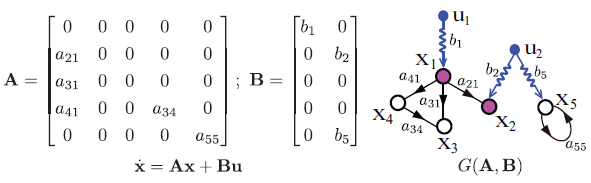
\includegraphics[scale=.55]{control}
		\end{column}
		\begin{column}{.4\textwidth}		
			\begin{itemize}
				\item B indicates which nodes are drivers
				\item $u(t)$ are the control inputs
			\end{itemize}
		\end{column}
	\end{columns}
	
	\begin{columns}
		\begin{column}{.5\textwidth}
			 $(A,B)$ is controllable if it can be steered from any initial state $ x_0 $ to any final state $ x_f $ with a sequence of inputs $u(t)$
		\end{column}
		\begin{column}{.5\textwidth}
			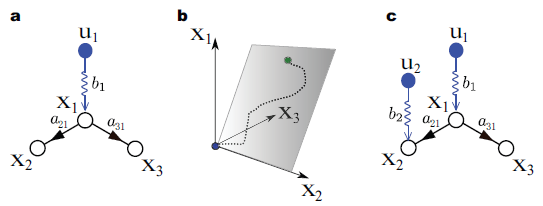
\includegraphics[scale=.55]{control2}
		\end{column}
	\end{columns}
	\begin{itemize}
		\item Can we determine if a system $(A,B)$ is controllable ?
		\item What is the minimum set to fully control the network ?
	\end{itemize}
	More information in \footfullcite{Liu2015}
\end{frame}

\begin{frame}
	\frametitle{Optimal control}
	
	\begin{columns}
		\begin{column}{.7\textwidth}
			\begin{itemize}
			\item There might exists multiple sequences of inputs $ u(t) $ that drives the system $(A,B)$ from $x_0$ to $x_f$
			\end{itemize}
		\end{column}
		\begin{column}{.3\textwidth}
			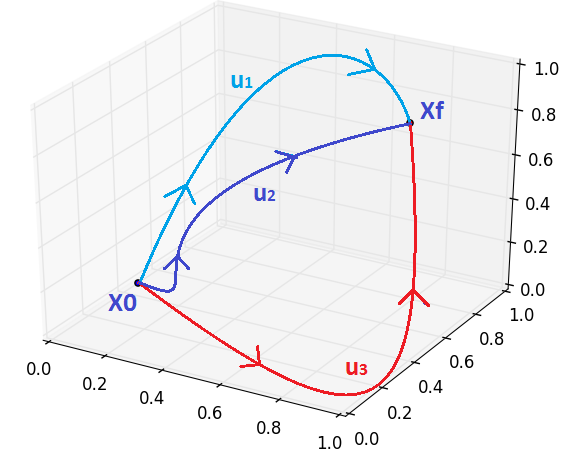
\includegraphics[scale=.3]{trajectories}
		\end{column}
	\end{columns}
	\begin{itemize}
		\item Optimal control : finding the one that minimizes some cost function
		\item Here we are concerned with the control energy : $ \mathcal{E} = \int_{t_0}^{t_f} \Vert u(t) \Vert^2 dt $
		\item The smallest this energy, the less stress on the storage devices
		\item It has been shown that :
		\begin{itemize}
			\item the control input sequence that minimizes the control energy can be written as $u^{\star}(t) =B^T(A^T)^{t_f-t-1}W^{-1}(t_f) \left[ x_f - A^{t_f}x_0 \right] $ \footfullcite{Summers2014}
			\item Where the gramian matrix $ W(t) = \sum_{k=0}^{t} A^kBB^T(A^T)^k $
			\item The control energy is then $ \mathcal{E}_{min}= \left[ x_f - A^{t_f}x_0 \right]^{T}W^{-1}(t_f)\left[ x_f - A^{t_f}x_0 \right] $
		\end{itemize}
	\end{itemize}
\end{frame}

\begin{frame}
	\frametitle{Gramian}
	
	\begin{itemize}
		\item Control energy depends on $W^{-1}$
		\item $W$ depends on A and B, but not on $x_0$ and $x_f$
		\item $W$ can be used to obtain average information :
		\begin{itemize}
			\item $rank[W] $ gives the dimension of the controllable subspace
			\item $Tr[W^{-1}]$ gives information about average control energy
		\end{itemize}
		\item Useful for us since the prosumers change a lot
		\item Goal : good performances (low control energy) on average
	\end{itemize}
	PROBLEMS :
	\begin{itemize}
		\item We still do not know how to find B (the driver nodes)
		\item We have constraints on line capacities, battery capacities and charge/discharge rates
	\end{itemize}
\end{frame}

\section{submodular set functions}
\begin{frame}
	\tableofcontents[currentsection]
\end{frame}

\begin{frame}
	\frametitle{Submodular set functions}
	
	\begin{columns}
		\begin{column}{.6\textwidth}
			\begin{itemize}
				\item Let $F:2^V \longrightarrow \Re$ be a set function
				\item F is submodular if for all sets $A,B \subset V$ such that $A \subseteq B$, and for all element $x \in V \ B $ : $ F(A \cup \{x\})-F(A) \geq F(B \cup \{x\})-F(B) $
				\item Diminishing returns
				\item Greedy heuristic with worst case guarantee : $\frac{F(S_{greedy})}{F(S_{opt})} \geq 63\%$
			\end{itemize}
			\begin{figure}		
				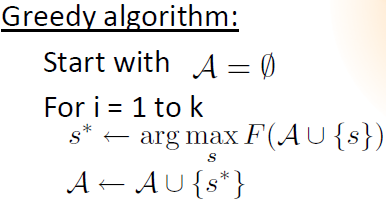
\includegraphics[scale=.5]{greedy}
			\end{figure}
	  	\end{column}
	  	\begin{column}{.4\textwidth}
	  		\begin{figure}
				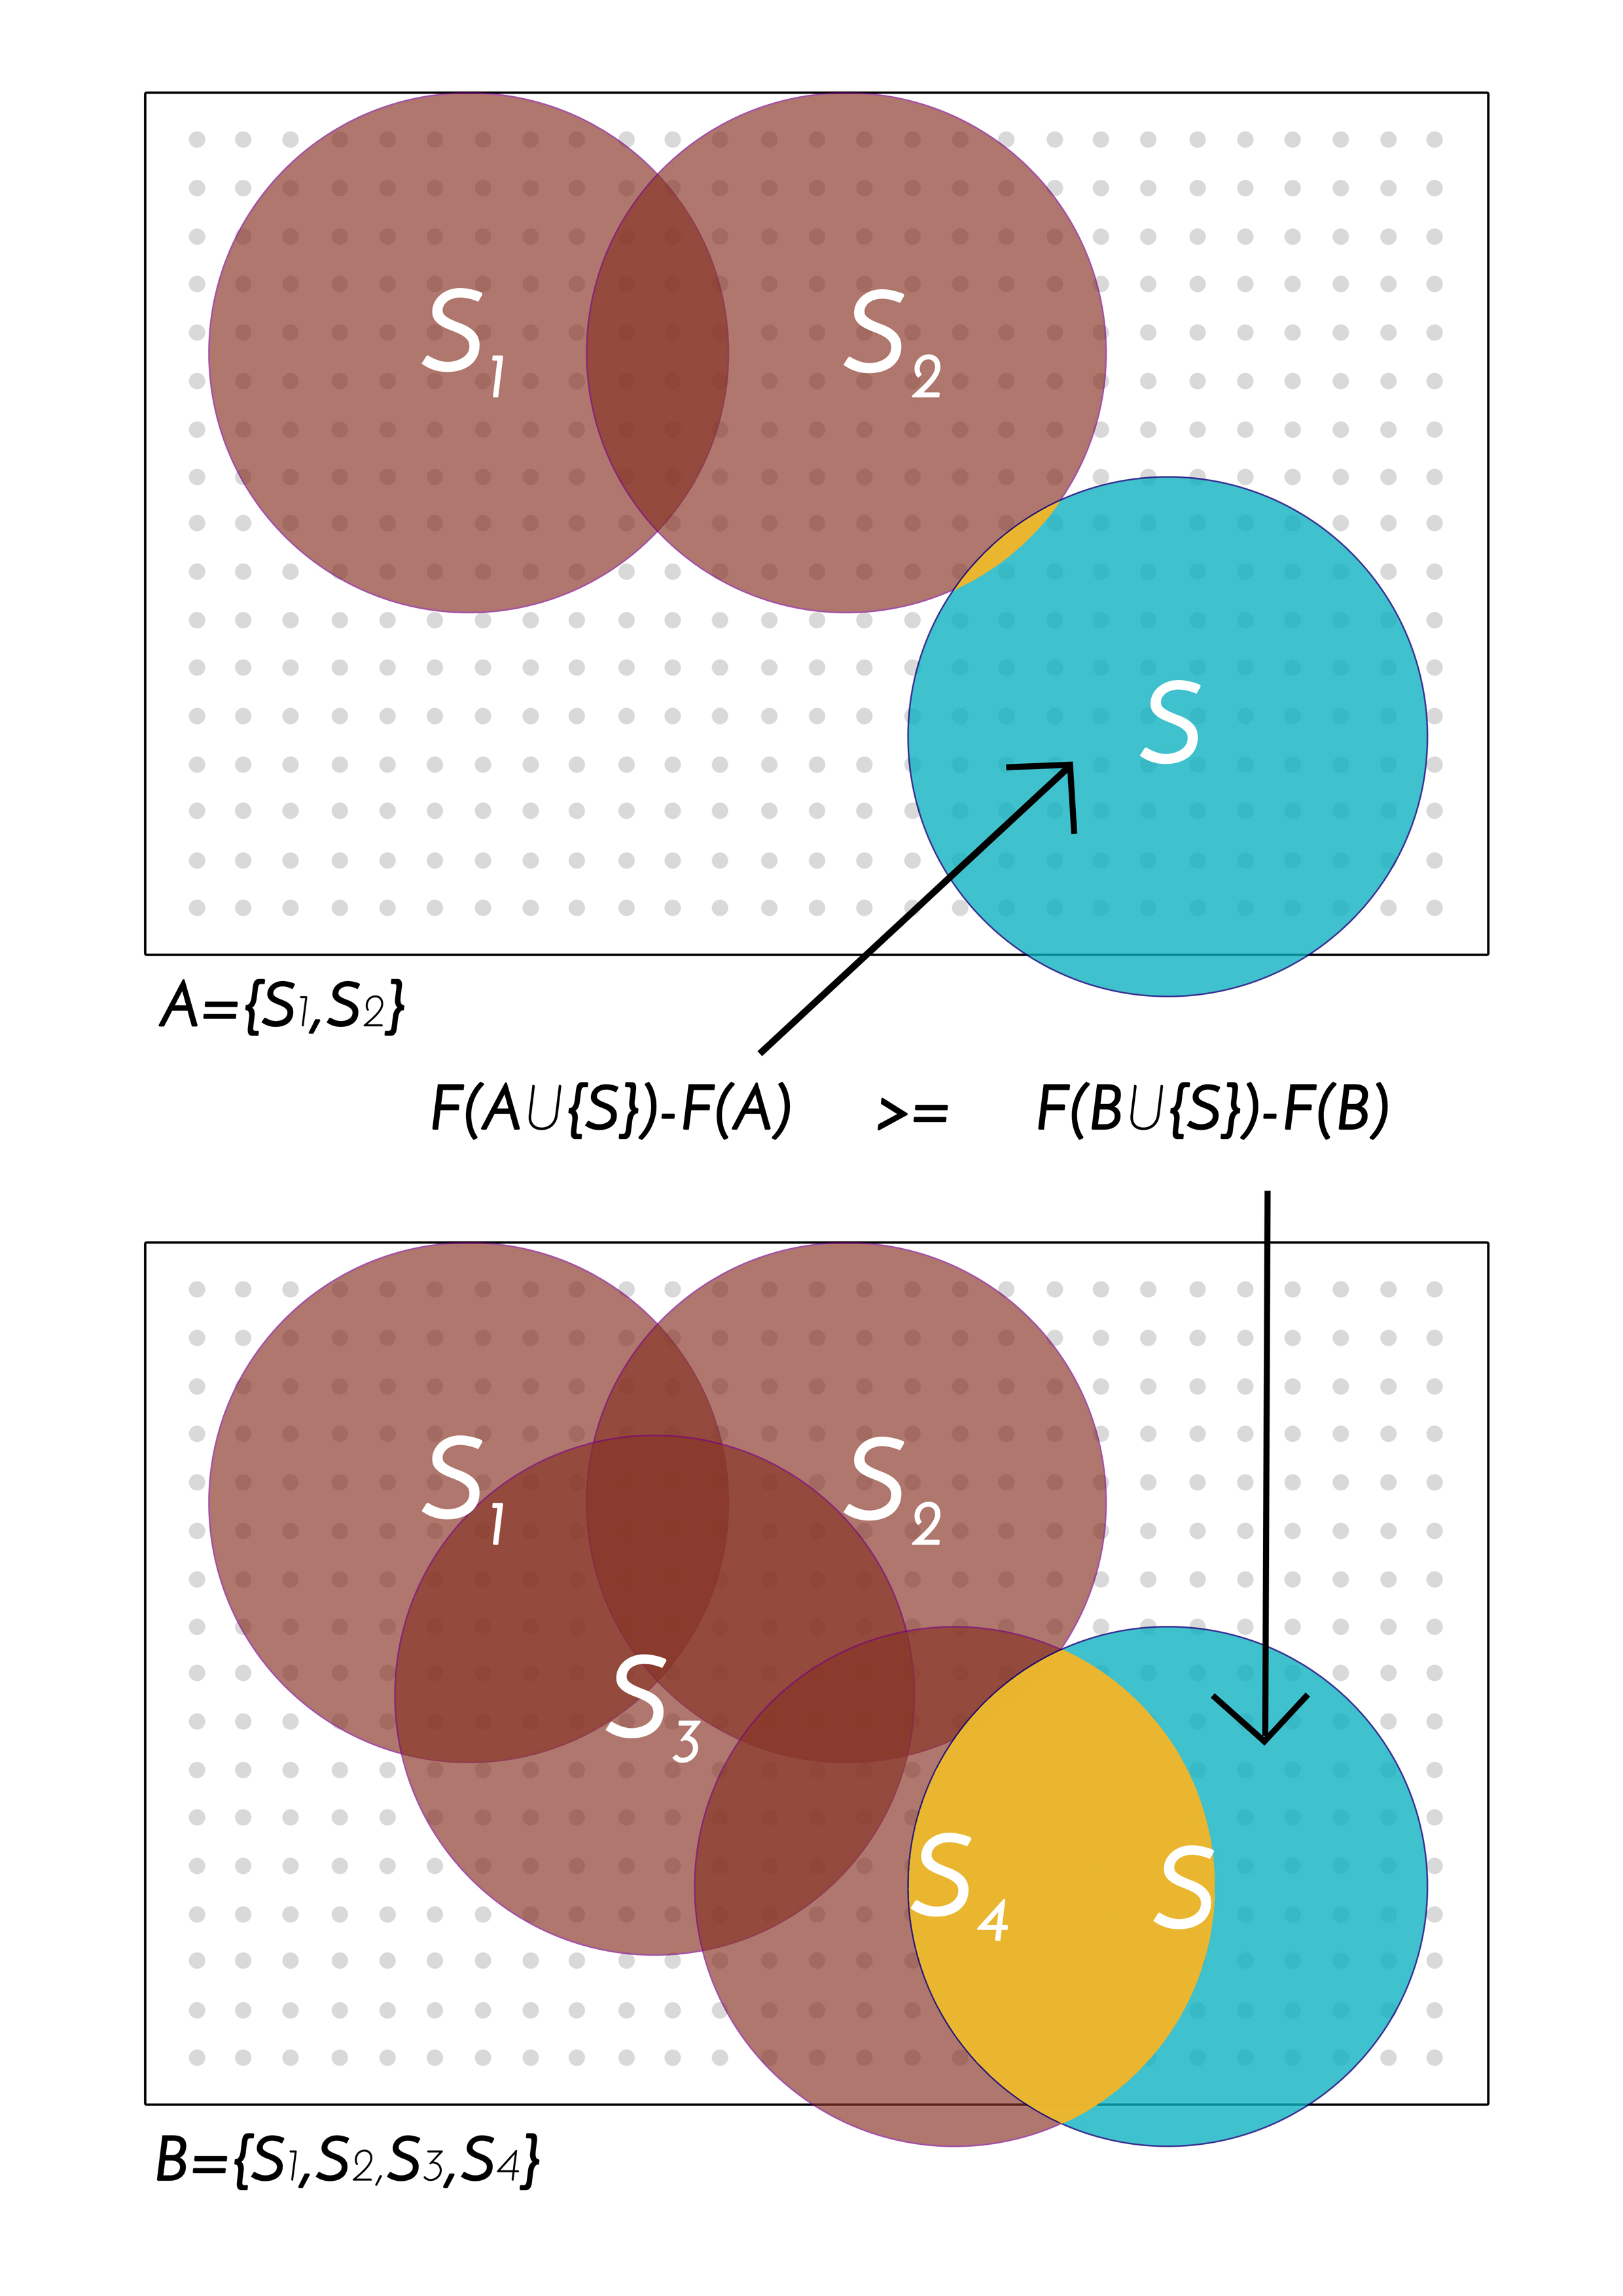
\includegraphics[scale=.25]{figure_1}
			\end{figure}	
		\end{column}
	\end{columns}
\end{frame}

\begin{frame}
	\frametitle{Gramian and Submodularity}

	What is the link between submodular set functions and controllability ?
	\begin{itemize}
		\item Let $B_S$ be matrix B when driver set is S
		\item $W_S $ : Gramian of system $ (A,B_S) $ 	
		\begin{itemize}
			\item $F_{trace}:S \longrightarrow Tr[W_S] $ is modular
			\item $F_{traceInv}:S \longrightarrow Tr[W_S^{-1}] $ is submodular
			\item $F_{rank}:S \longrightarrow rank[W_S] $ is submodular
		\end{itemize}	
	\end{itemize}

	More information and demonstrations in \footfullcite{Summers2014}
	
	More information about submodularity and maximization of submodular set functions in \footfullcite{Krause2014}	
\end{frame}

\section{Some results}
\begin{frame}
	\tableofcontents[currentsection]
\end{frame}

\begin{frame}
	\frametitle{Combining the pieces}

%	\begin{itemize}
%				\item System state at t : $ Y(t) = \{ \theta_1,\theta_2,...,\theta_N,\dot{\theta}_1,\dot{\theta}_2,...,\dot{\theta}_N,1\} $
%				\item Dynamics : $ Y(t+\Delta t) = A Y(t) + B u(t) $
%				\item Energy : $ \mathcal{E}_{min}= \left[ x_f - A^{t_f}x_0 \right]^{T}W^{-1}(t_f)\left[ x_f - A^{t_f}x_0 \right] $
%				\item Submodular function $F(S) = Tr[W_S^{-1}]$
%	\end{itemize}

	
	
	\begin{columns}
		\begin{column}{.5\textwidth}
			\begin{figure}
		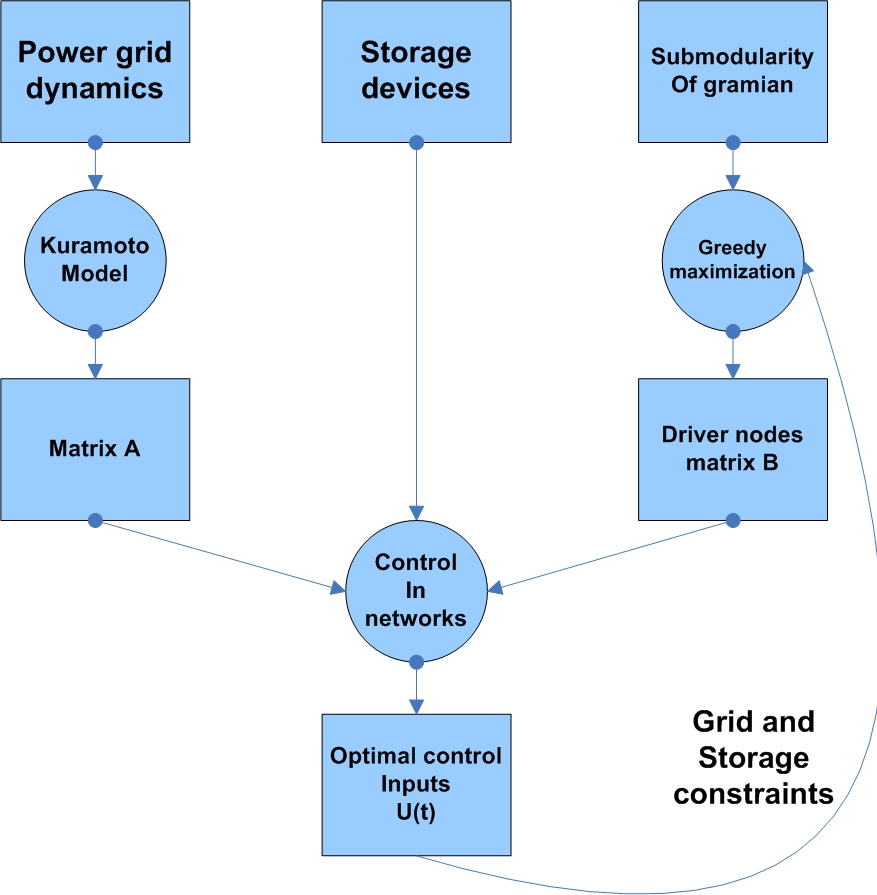
\includegraphics[scale=.3]{recap}
	\end{figure}
%				Constraints :
%				\begin{itemize}
%					\item Flow constraints %: $ \forall (i,j) \in V^2, \forall t,\ g_{ij} \vert \theta_j(t) - \theta_i(t) \vert \leq 1 $
%					\item Synchronization constraint %: $ \Vert (L \circ P^{MAX})^{\dagger} \Psi \Vert_{\infty} \leq sin(1) $
%					\item Balance constraint %: $ \sum_{k=1}^{N}P_{S,k} = 0 $
%					\item Battery levels constraints %: $ \forall t - \frac{\Lambda(0)}{I\Omega} \leq - \sum_{k=0}^{t}u^{\star}(k) \leq \frac{\Lambda_{MAX}-\Lambda(0)}{I\Omega} $
%					\item Charge/discharge rate constraints %: $\forall t, \vert u^{\star}(t)I\Omega \vert \leq r $
%				\end{itemize}
		\end{column}
		\begin{column}{.5\textwidth}
			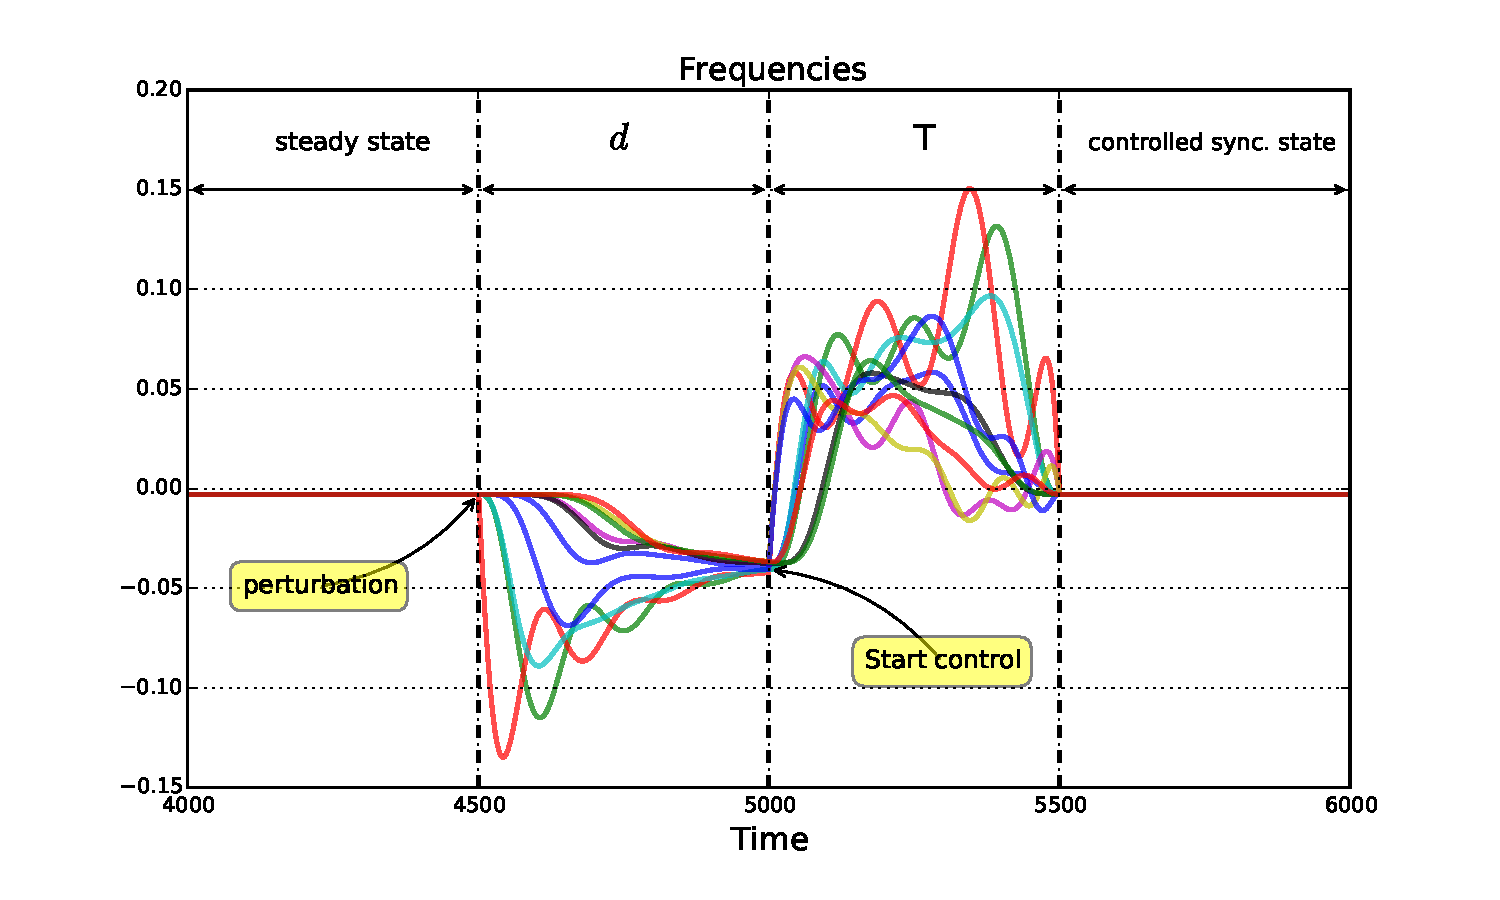
\includegraphics[scale=.27]{figure_2}
		\end{column}
	\end{columns}
\end{frame}

\begin{frame}
	\frametitle{Control energy}
	
	Are we doing better than random ?
	\begin{columns}
		\begin{column}{.6\textwidth}		
			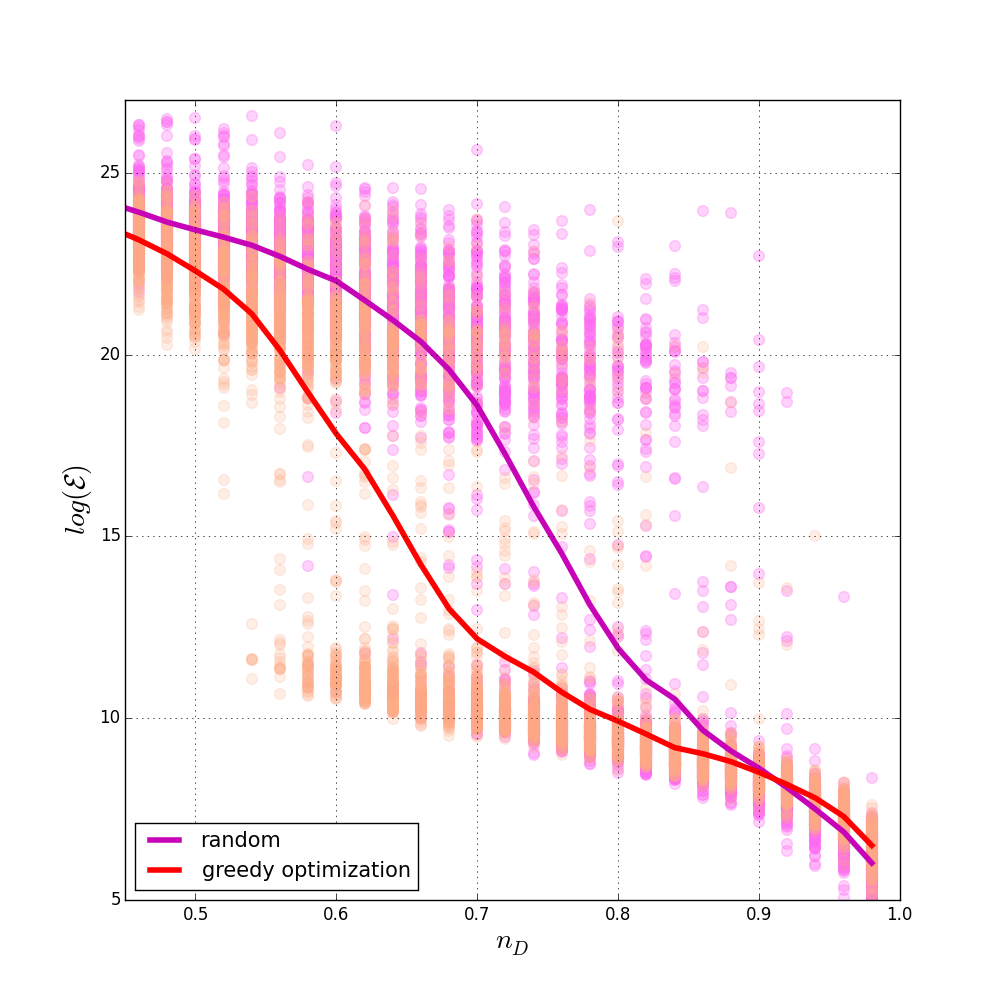
\includegraphics[scale=.3]{figure_3.png}
		\end{column}
		\begin{column}{.4\textwidth}
			\begin{itemize}
				\item Random scale-free topologies (200 nodes)
				\item Random power distributions and line capacities
			\end{itemize}
		\end{column}
	\end{columns}
	
\end{frame}



\begin{frame}
	\frametitle{real topology}
	
	{\footnotesize European transmission power grid (1494 nodes and 2196 edges over 25 countries) \footfullcite{jensen_2015_35177}}
	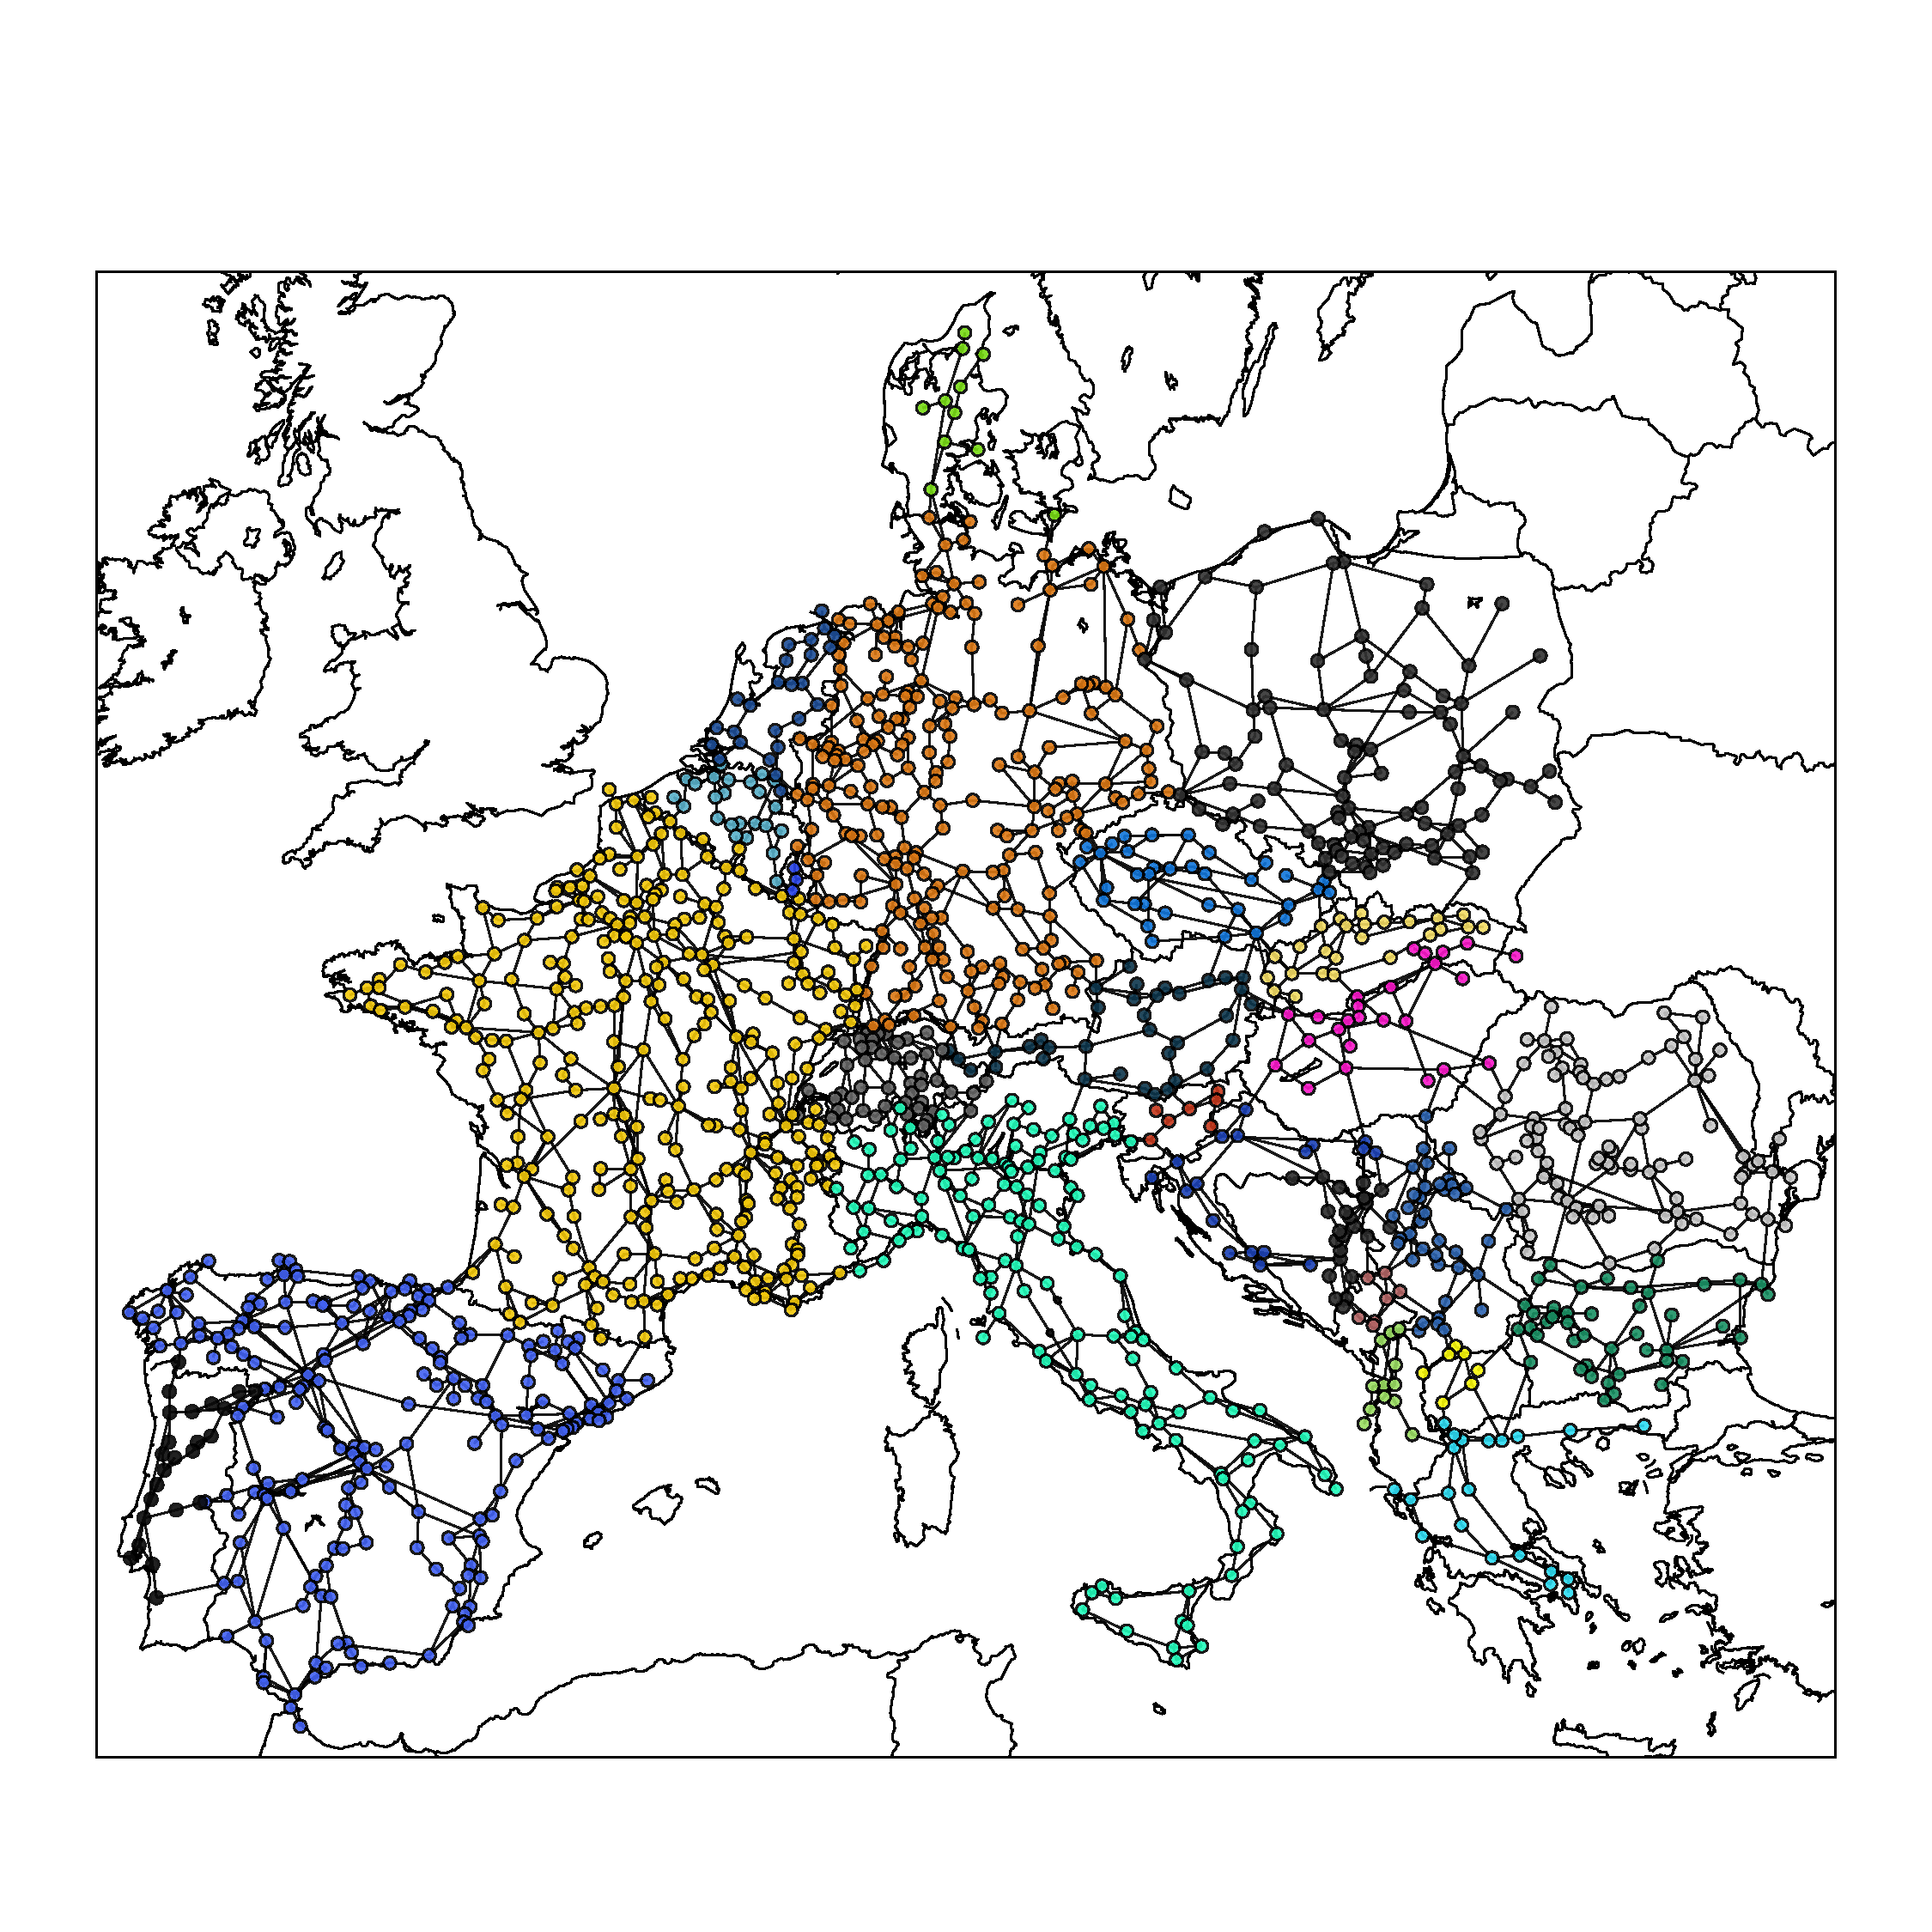
\includegraphics[scale=.165]{power_grid}
	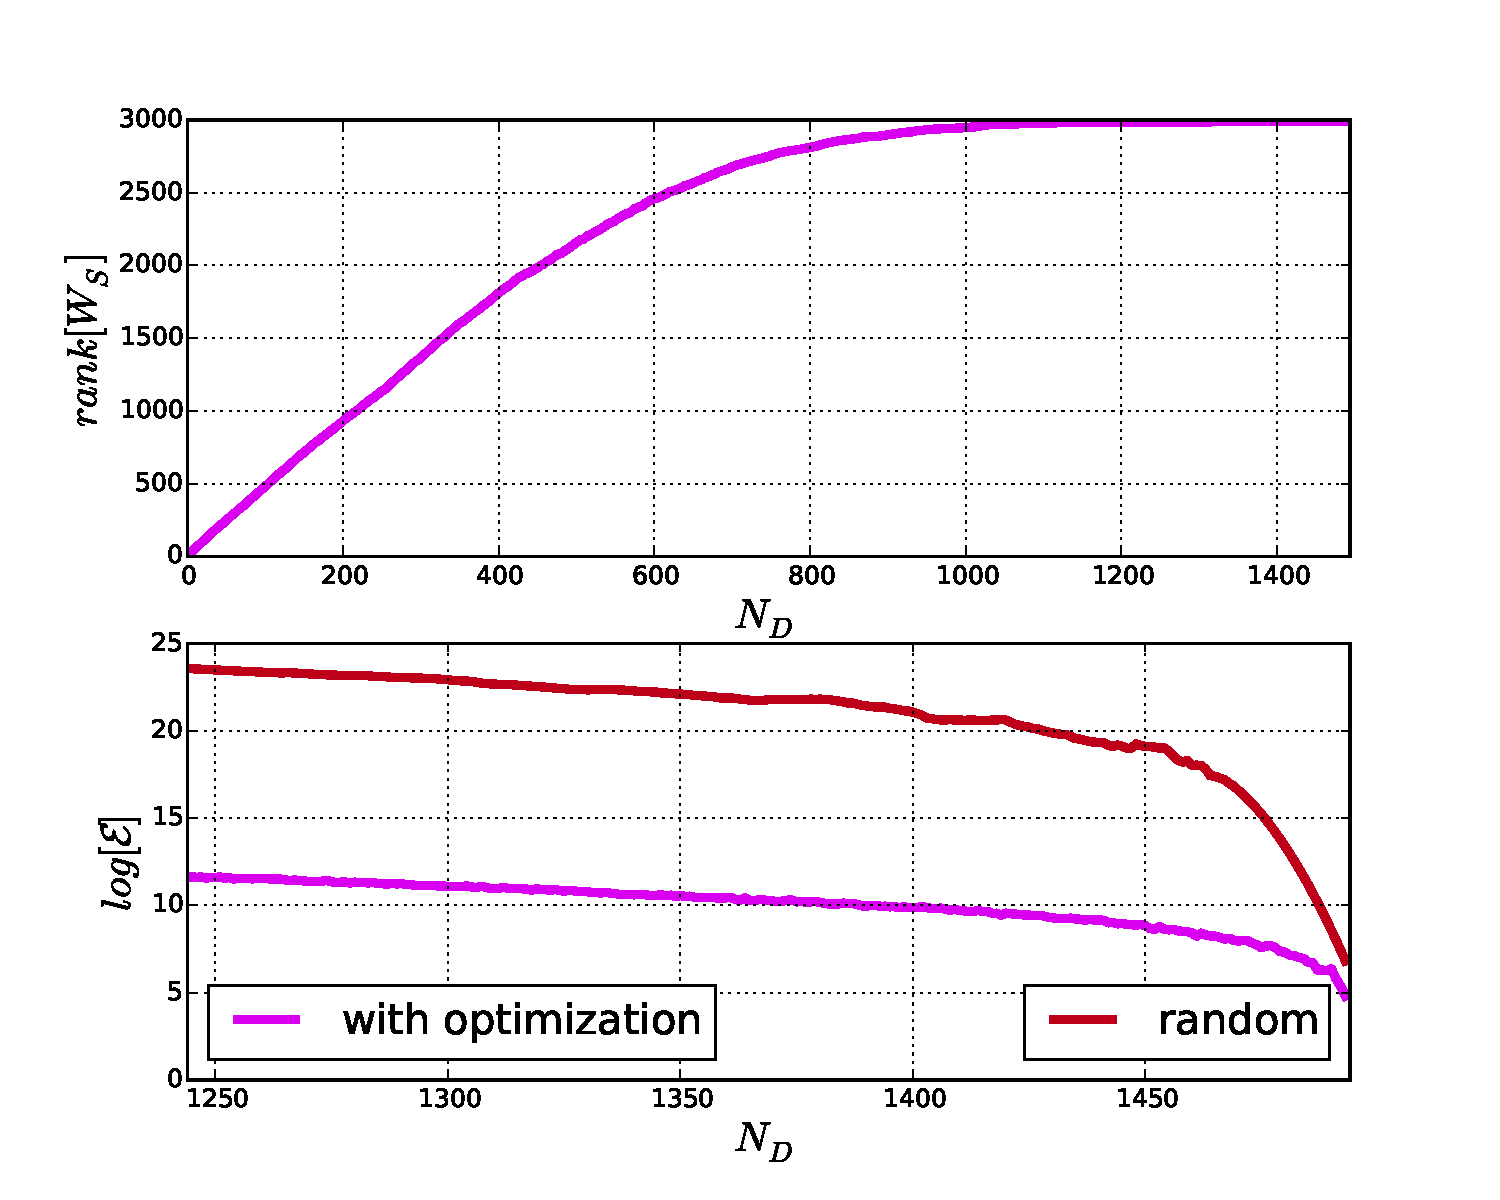
\includegraphics[scale=.26]{figs2}
\end{frame}

\begin{frame}
	\frametitle{Questions ?}
	
	\begin{center}
		Thank you for your attention. Questions ?
	\end{center}
\end{frame}

\begin{frame}
	\frametitle{Control and topology}
	
	How does the topology impact the size of the driver set ?	
	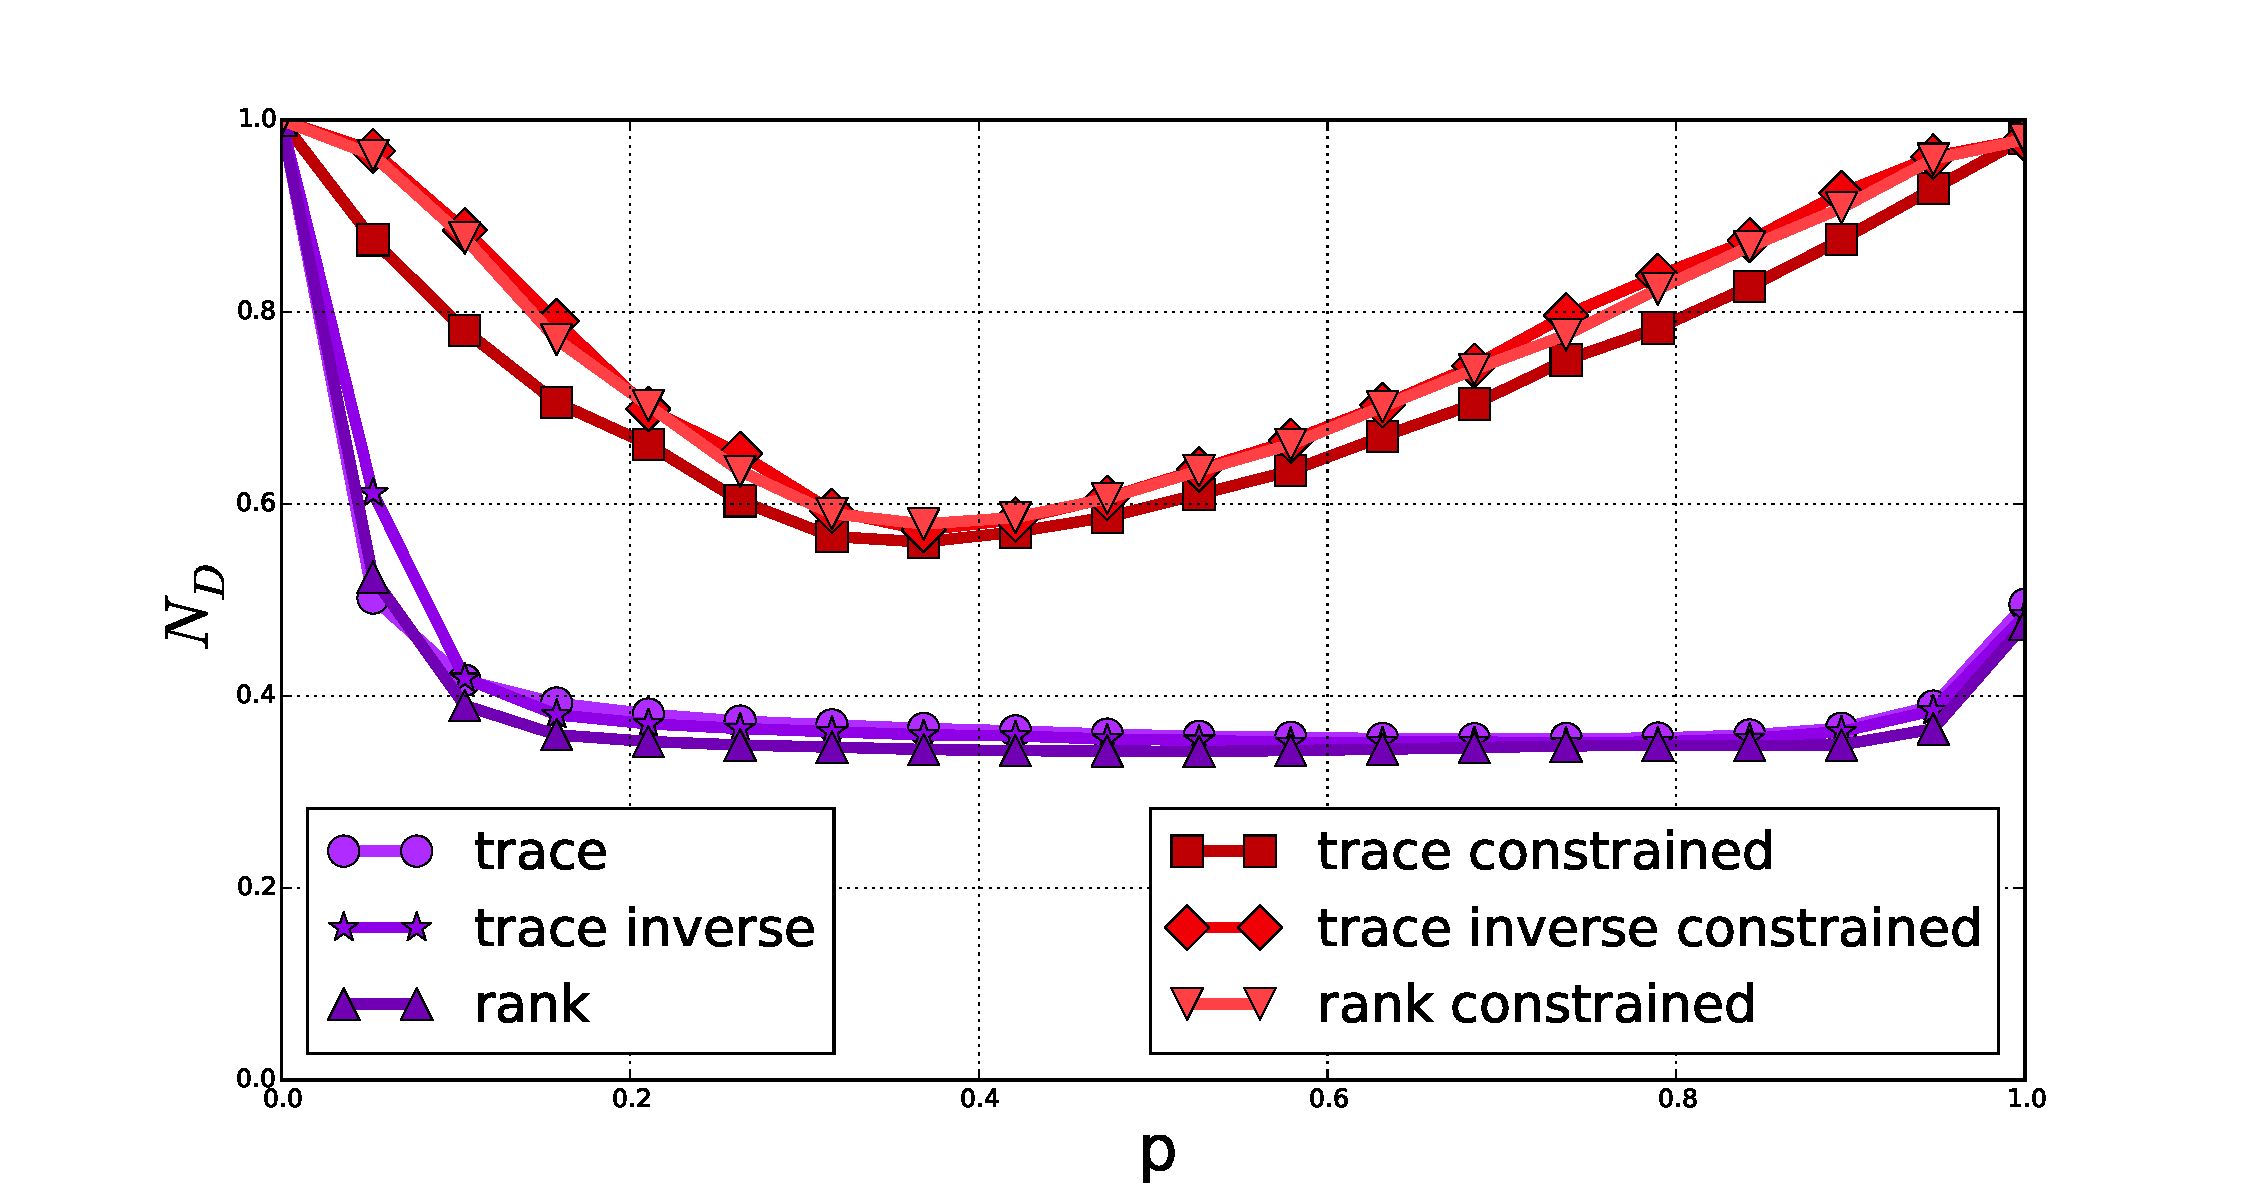
\includegraphics[scale=.3]{figure_4}
	\begin{itemize}
		\item Random erdos-renyi topologies (200 nodes)
		\item Random power distributions and line capacities
	\end{itemize}
\end{frame}

\begin{frame}
	\frametitle{Control and capacity distribution}
	
	How does the capacity distribution of the batteries impact the size of the driver set ?
	
	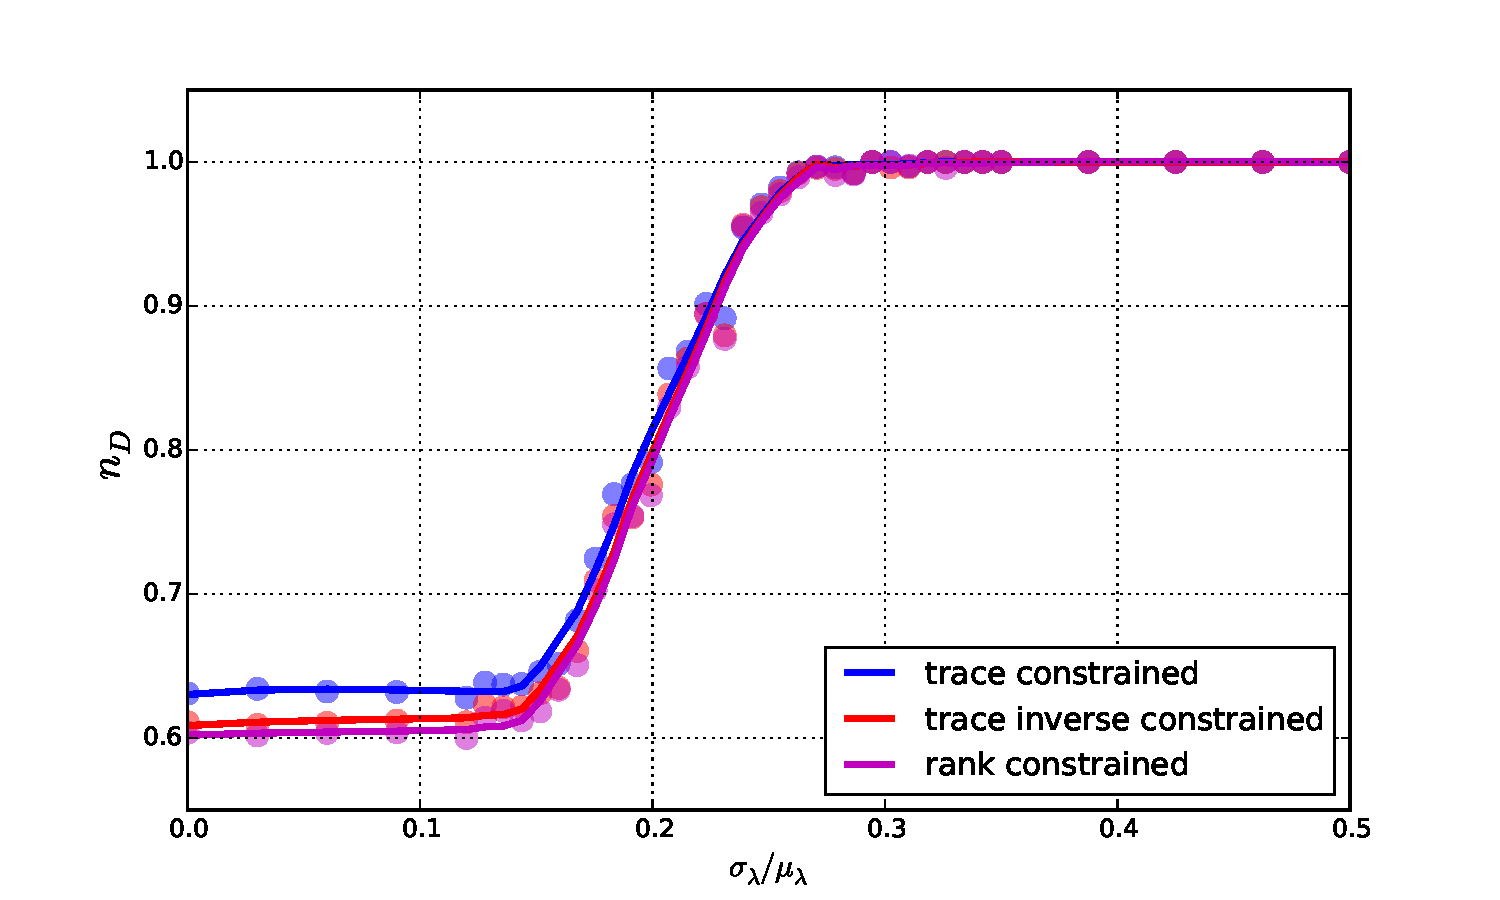
\includegraphics[scale=.3]{figure_7}
	\begin{itemize}
		\item Random erdos-renyi topologies (200 nodes)
		\item Random power distributions and line capacities
		\item Battery capacities are drawn from : $\mathcal{N}(\mu_{\lambda}, \sigma_{\lambda})$
	\end{itemize}
\end{frame}

\end{document}
